\documentclass{jhwhw}
%\usepackage{cite}
\usepackage{amsmath,amssymb}
\usepackage{graphicx,float}
%\usepackage[margin=1in]{geometry}
\usepackage{hyperref}

\renewcommand\thesubsection{\roman{subsection}}

\title{ISM Course: Assignment 3}
\author{V PremVijay}

\begin{document}

\maketitle

%\begin{abstract}
%In this work, 
%
%\end{abstract}


\problem
{Free-Free emission from the HII region}
%Radio continuum emission from a HII region at a distance 5.7 kpc from us is given in the table below.Observed size (diameter) of this HII region is 0.6” and radio recombination lines suggest a gas kinetic temperature of 7000 K. Find the emission measure and electron density of this HII region. If the star is a typical O star what can you say about the measured size.
%~\\



\solution
%\begin{figure}[H]
%	\centering
%	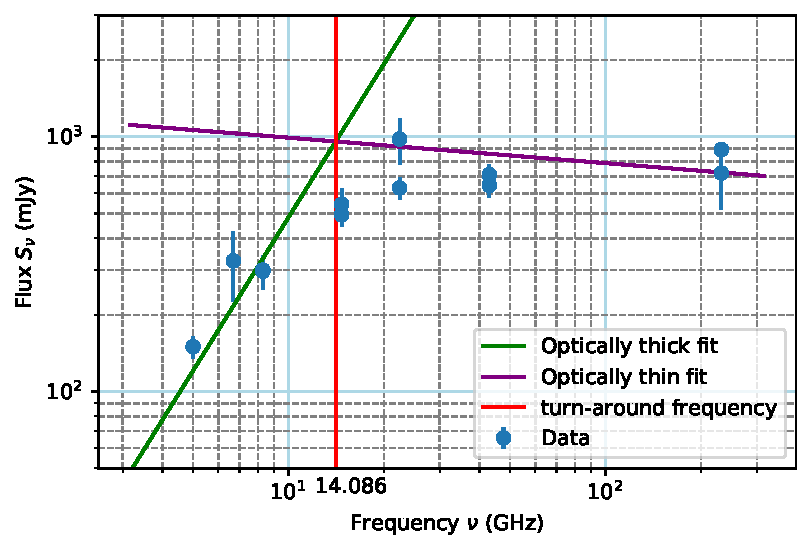
\includegraphics[width=1\linewidth]{../prob-1}
%	\caption{}
%	\label{fig:prob-1}
%\end{figure}

The given flux density at different frequency can be used to plot SED of the HII region. Uncertainties are unknown for some measurements, so let us consider a large uncertainty to those.
\begin{figure}[H]
	\centering
	\label{fig:prob-1-plot1}
	\caption{SED data of G28.20-0.04 N}
	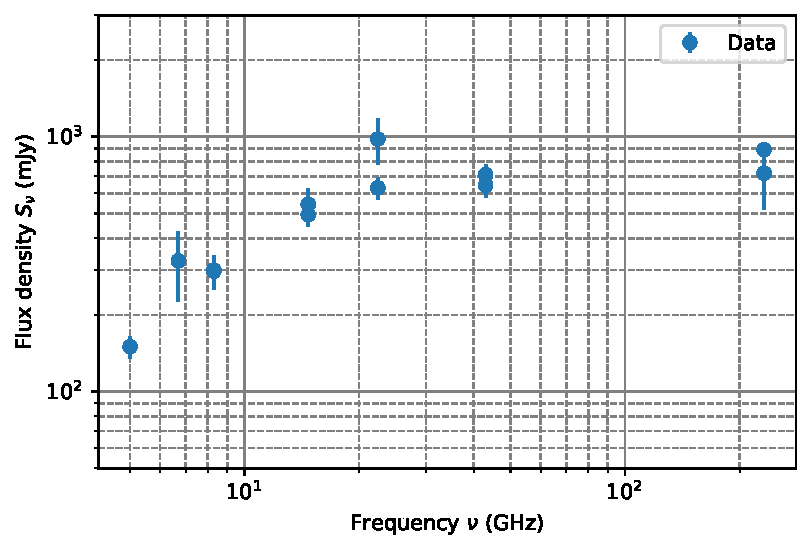
\includegraphics[width=1\linewidth]{../prob-1-plot1}
\end{figure}
In the log-log plot above\ref{fig:prob-1-plot1}, we can see that the flux increases with frequency in one regime and decreases with frequency in another regime. These are the optically thick and optically thin regimes.\\
For free-free emission in the radio frequencies, the optical depth is
\begin{align}
\label{prob-1-tau}
\tau_{\nu} &= 8.24 \times 10^{-2} T^{-1.35} \nu^{-2.1} E_{c} 
\end{align} 
where $E_{c}$ is emission measure in cm$^{-6}$ pc, $\nu$ is frequency in Hertz and $T$ is temperature in Kelvin.


Applying the radiative transport equation, we get $I_{\nu} \propto \nu^2$ in the optically thick regime and $I_{\nu} \propto \nu^{-0.1}$ in the optically thin regime, assuming no background source in this frequency range. We can now fit the data by these power laws in the two regime. I use a curve fitting algorithm that accounts for uncertainties. Then the frequency  at the intersection between the two fitting curves is considered as the turn-around frequency $\nu_{0}$.


\begin{figure}[H]
\centering
\caption{Optically thick and thin regimes}
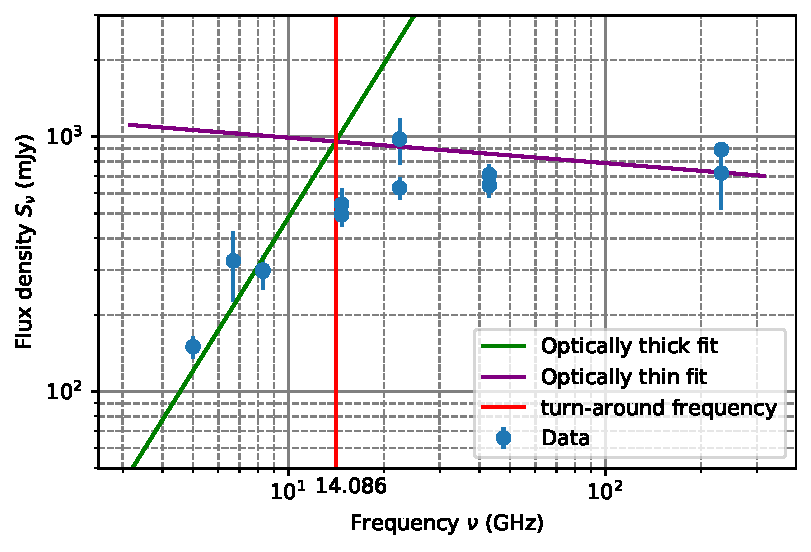
\includegraphics[width=1\linewidth]{../prob-1-plot2}
\label{fig:prob-1-plot2}
\end{figure}


The optical depth at the turn-around frequency is $\tau_{\nu_{0}} \sim 1$. From the above figure we can get $\nu_{0}=14.086$ GHz. Inserting this in the equation \ref{prob-1-tau}, we can get the emission measure as we know the temperature is $T=7000$ K.
\begin{align}
E_c = \frac{T^{1.35} \times \nu_0^{2.1}}{8.24 \times 10^{-2}} = 4.87 \times 10^{8} ~\rm{pc ~cm^{-6}}
\end{align}
Emission measure is the integration along line of sight,
\begin{align}
E_c = \int n_+ n_e ds
\end{align}
The HII region is at a distance of 5.7 kpc, and its angular size is only $0.6''$. This gives its size as 0.0166 pc, hence it is an hypercompact HII region. We can find the electron density in this region by assuming it is constant and equal to ion density within this region. This is likely a very good assumption based on what we saw in cloudy simulation. Let us consider the average length of HII region along the line of sight to be half of the size. This gives
\begin{align}
n_e = 2.42 \times 10^5 ~\rm{cm^{-3}}
\end{align}
We have already computed HII region size as a function of density using cloudy in the last assignment. By comparing with that, we can say that a typical O star has to be much larger to sustain such a dense HII region of that size. Hence it is likely a protostar.






\problem{N(HI) and metallicity estimate}






\solution
From the results obtained in assignment 1, we can say that this ISM is optically thin
for the 21 cm emission line. Hence we can obtain the column density from the 21cm emission line spectrum using the relation,
\begin{align}
\int \left( T_A - T_A(0)\right)  du = 54.89 \times \rm{K~ km/s} ~\frac{N(HI)}{10^{20} \rm{cm^{-2}}} 
\end{align}
%

\begin{figure}[H]
\centering
\caption{Spectrum of 21 cm emission line}
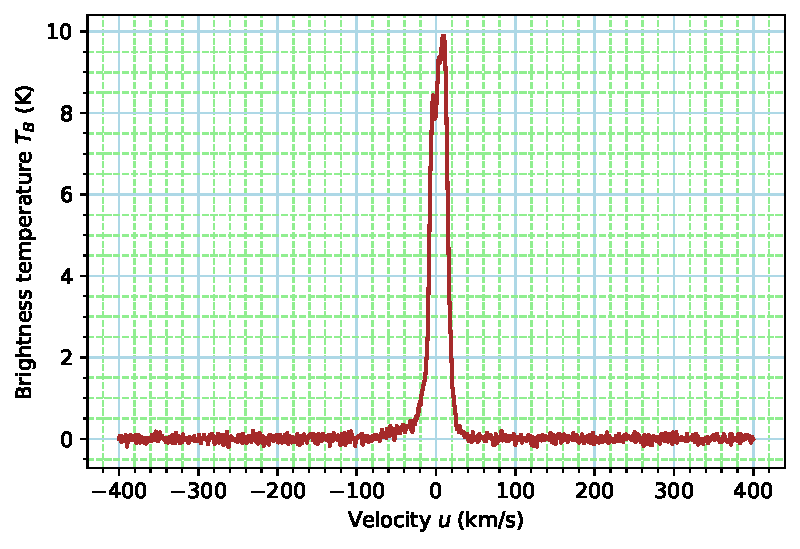
\includegraphics[width=1\linewidth]{../prob-2-plot1}
\label{fig:prob-2-plot1}
\end{figure}



The given spectrum is just integrated over velocity to get
$\rm{N(HI_{21cm}) = 4.73 \times 10^{20} cm^{-2}}$.
%
The column density obtained by Voigt profile to Lymen-$\alpha$ is 
$\rm{N(HI_{Ly \alpha}) = 7.126 \times 10^{20} cm^{-2}}$.
They are not exactly equal, this might be because of multiple components in the line of sight. In the figure above, we an see that there are three peaks.\\

\newpage
\noindent
The column densities obtained in the assignment-1 are
\begin{table}[H]
\centering
\begin{tabular}{l|l}
ID & Column density N (cm$^{-2}$)\\
\hline & \\
FeII  & 1.778e+15 \\
NiII  & 1.400e+14 \\
SII   & 2.044e+15 \\
SiII  & 1.371e+14 \\
SiIII & 3.192e+13 \\
SiIV  & 5.888e+13 \\
\end{tabular}
\end{table}

We can see that the singly ionized state is the dominant ionized state in Silicon. Assuming the same to be true for all the above elements, we get


\begin{table}[H]
\centering
\begin{tabular}{l|l|l|l|l}
ID & Abundance & Log10(Abundance) & Metallicity, Z$_{\rm{ISM}}$ & Metallicity, Z$_{\rm{Sun}}$\\
\hline & & & &\\
HI & 1.000e+00 & 0.000 & 0.000 & 0.000\\
FeII & 2.495e-06 & -5.603 & 0.597 & -1.103\\
NiII & 1.965e-07 & -6.707 & 1.033 & -0.927\\
SII & 2.868e-06 & -5.542 & -1.053 & -0.663\\
SiII & 1.924e-07 & -6.716 & -1.215 & -2.226\\
\end{tabular}
\end{table}

Z$_{\rm{ISM}}$ is the metallicity with respect to ISM abundance and Z$_{\rm{Sun}}$ is the metallicity with respect to solar abundance. We can see that the abundance of Fe and Ni are inbetween their respective solar and ISM abundances. But the Z$_{\rm{ISM}}$ of Si and S are very close, suggesting those lines are from ISM only.








\problem{Ionization and fine-structure excitation of C}






\solution
The column densities (in log
units, cgs) of C I, C II and CII* measured towards the star HD 185418 are
15.60, 17.80 and 14.90 respectively. Hence
%\begin{align}
%N(CI) = 
%\end{align}

\subsubsection{CI-CII}
Under ionisation equilibrium between CI and CII, we have
\begin{align}
\frac{N(CI)}{N(CII)} &= \frac{n_e \alpha(T)}{\Gamma_{CI}}\\
10^{(15.6-17.8)} &= n_e  \times\frac{ 9.5 \times 10^{-12} ~\rm{cm^3s^{-1}}}{2.1 \times 10^{-10} ~\rm{s}^{-1}} \left(  \frac{T}{100 ~K} \right)^{-0.6}
\end{align}
where we have ignored the dust extinction.

\begin{figure}[H]
\centering
\caption{Electron density-Temperature constraint from CI:CII ratio}
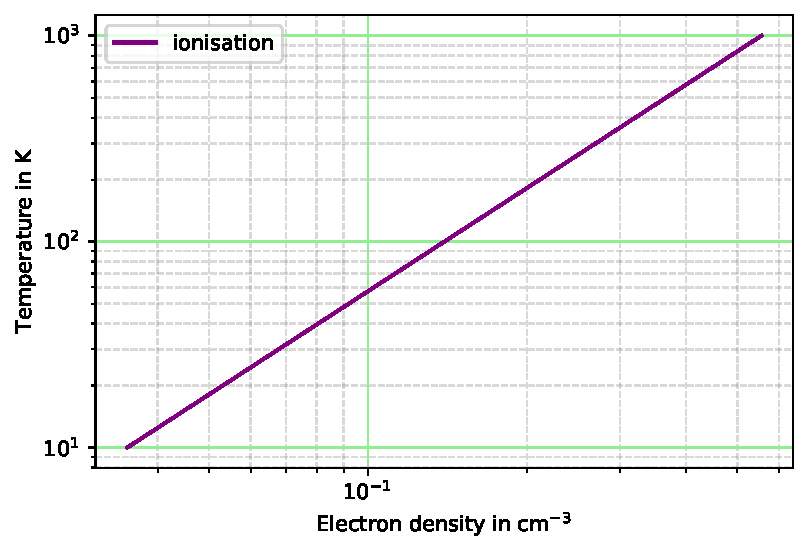
\includegraphics[width=1\linewidth]{../prob-3-plot-1}
\label{fig:prob-3-plot-1}
\end{figure}

\subsubsection{CII-CII*}
Under fine-structure excitation equilibrium between CII and CII*, we have
\begin{align}
\frac{N(CII*)}{N(CII)} &= \frac{Q_{12}(e) n_e + Q_{12}(H) n_H + \Gamma_R + \Gamma_{UV}}{A_{21}}\\
10^{(14.9-17.8)} &=  \frac{[Q_{12}(e) + Q_{12}(H) \times 1000] ~n_e + \Gamma_R + \Gamma_{UV}}{A_{21}}
\end{align}
where we assumed a ion fraction, to write hydrogen density in terms of electron density. 
\begin{figure}[H]
	\centering
	\caption{Electron density-Temperature constraint from CII:CII* ratio}
	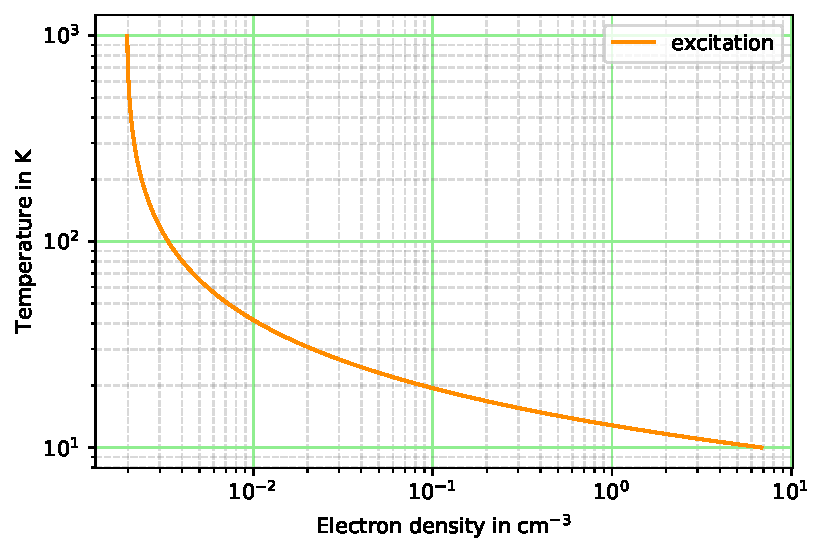
\includegraphics[width=1\linewidth]{../prob-3-plot-2}
	\label{fig:prob-3-plot-2}
\end{figure}

\newpage
\subsubsection{Consistent solution}
The consistent solution is at the insersection of two constraint curves.
\begin{figure}[H]
\centering
\caption{Consistent values for electron density and temperature}
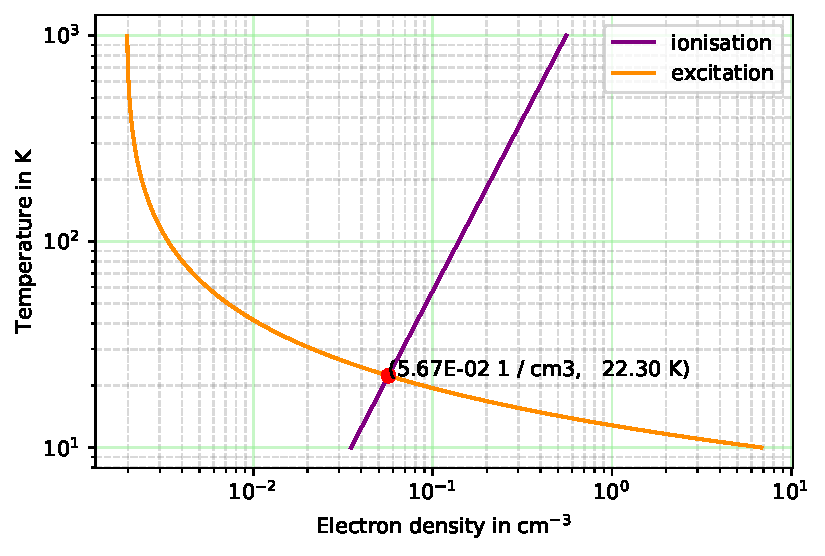
\includegraphics[width=1\linewidth]{../prob-3-plot-3}
\label{fig:prob-3-plot-3}
\end{figure}
Hence we have a consistent solution for ionisation and fine-structure excitation,
\begin{align}
T &= 22.30 ~\rm{K}\\
n_e &= 5.67 \times 10^{-2} ~\rm{cm^{-3}}
\end{align}















\problem{Simple estimates using $H_2$ column densities}






\solution
\subsection{H$_2$ molecular fraction in the cloud}
H2 molecular fraction is 
\begin{align}
\frac{2~N(\rm{H_{2}})}{N(\rm{HI}) + 2~N(\rm{H_{2}})} = 0.446
\end{align}

\subsection{Temperature of the gas using T 01}

\begin{align}
\frac{N(J=1)}{N(J=0)} &= 9 \exp \left( \frac{-170.5 ~\rm{K}}{T_{01}} \right)\\
\implies T_{01} &= \frac{170.5 ~\rm{K}}{\ln[9 N(J=0)/N(J=1)]} = 98.17  ~\rm{K}
\end{align}

\subsection{The excitation diagram}

Degeneracy factor is
\begin{align}
g_J = \begin{cases}
3(2J+1) ~ \text{for odd} ~J\\
2J+1 ~~~~\text{for even} ~J
\end{cases}
\end{align}

\begin{figure}[H]
	\centering
	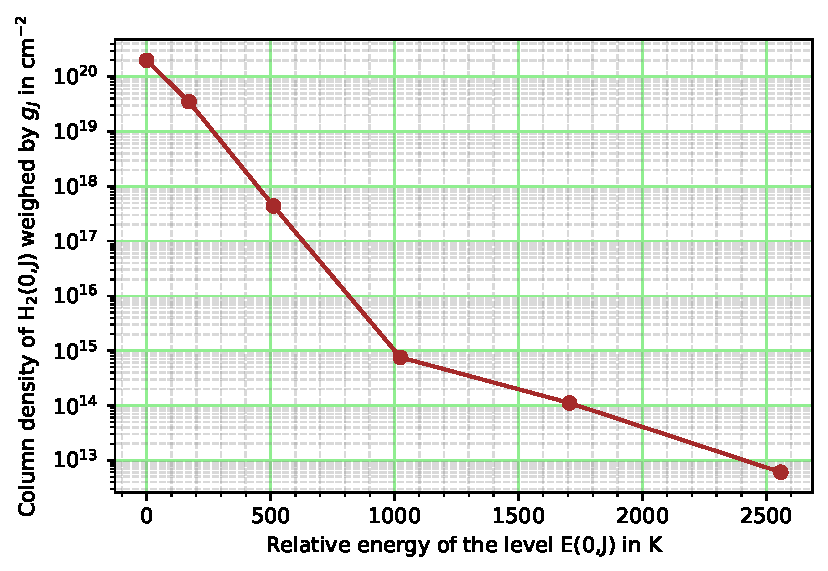
\includegraphics[width=.9\linewidth]{../prob-4-plot-1}
	\label{fig:prob-4-plot-1}
	\caption{Excitation diagram of H$_2$ rotation levels.}
\end{figure}


\subsection{Estimating $\beta(0)$}
Under equilibrium we have,
\begin{align}
\label{prob-4-beta-0}
p_{4,0} ~\beta(0) ~n(H_2,J=0) + 0.19 ~R n(H)n &= A(4\to 2) ~n(H_2,J=4)\\
\label{prob-4-beta-1}
p_{5,1} ~\beta(1) ~n(H_2,J=1) + 0.44 ~R n(H)n &= A(5\to 3) ~n(H_2,J=5)
\end{align}
and
\begin{align}
R n(H)n &= 0.11 \sum_{J=0}^{6} \beta(J) ~n(H_2,J)
\end{align}
Just for estimation let us assume that $\beta(J)=\beta(0)$ for all J. Hence eq. \eqref{prob-4-beta-0} becomes,
\begin{align}
\label{prob-4-beta-0-1}
p_{4,0} ~\beta(0) ~n(H_2,J=0) + 0.19 ~(0.11) \sum_{J=0}^{6} \beta(0) ~n(H_2,J) &= A(4\to 2) ~n(H_2,J=4)\\
\beta(0) \left[ p_{4,0} ~n(H_2,J=0) + 0.19 ~(0.11) \sum_{J=0}^{6} ~n(H_2,J) \right] &= A(4\to 2) ~n(H_2,J=4)\\
\implies \beta(0) \left[ p_{4,0} ~n(H_2,J=0) + 0.19 ~(0.11) ~n(H_2) \right] &= A(4\to 2) ~n(H_2,J=4)\\
\implies \beta(0) \left[ p_{4,0} ~N(H_2,J=0) + 0.19 ~(0.11) ~N(H_2) \right] &= A(4\to 2) ~N(H_2,J=4)
\end{align}
Putting $p_{4,0} = 0.26$ and $A(4\to 2) = 2.76 \times 10^{-9} s^{-1}$, we get 
\begin{align}
\beta(0) &= 4.40 \times 10^{-14} s^{-1}
\end{align}
%
%
Similarly by putting $\beta(J)=\beta(1)$ in eq. \eqref{prob-4-beta-1},
\begin{align}
\label{prob-4-beta-1-1}
p_{5,1} ~\beta(1) ~n(H_2,J=1) + 0.19 ~(0.11) \sum_{J=0}^{6} \beta(1) ~n(H_2,J) &= A(5\to 3) ~n(H_2,J=5)\\
\beta(1) \left[ p_{5,1} ~n(H_2,J=1) + 0.19 ~(0.11) \sum_{J=0}^{6} ~n(H_2,J) \right] &= A(5\to 3) ~n(H_2,J=5)\\
\implies \beta(1) \left[ p_{5,1} ~n(H_2,J=1) + 0.19 ~(0.11) ~n(H_2) \right] &= A(5\to 3) ~n(H_2,J=5)\\
\implies \beta(1) \left[ p_{5,1} ~N(H_2,J=1) + 0.19 ~(0.11) ~N(H_2) \right] &= A(5\to 3) ~N(H_2,J=5)
\end{align}
Putting $p_{5,1} = 0.12$ and $A(5\to 3) = 9.83 \times 10^{-9} s^{-1}$, we get 
\begin{align}
\beta(1) &= 3.11 \times 10^{-14} s^{-1}
\end{align}
In both ways we estimate a closely similar value for $\beta(0)$, so it justifies our assumption.










\problem{Isothermal shock}






\solution
The shock speed is $V_S = 100$~km/s.\\
Pre-shocked atomic hydrogen density is $n_0 = 100 ~$cm$^{-3}$.\\
After the shock passes, the velocity of the gas with respect to shock is
\begin{align}
u_S = \frac{1}{4} V_S = 25 \rm{km/s}
\end{align} 
and the density of the gas becomes
\begin{align}
n_S = 4 {n_0} = 400 ~\rm{cm^{-3}}
\end{align}
%
The temperature of the gas immediately after the shock passes is,
\begin{align}
T_S = \frac{3 \mu m}{16 k_B} \times V_S^2
\end{align}
Putting $\mu = 1$ for atomic hydrogen, we get $T_S = 2.26 \times 10^5$~K.\\
Hence the energy density of that gas is
\begin{align}
E = 3 k_B T n_S = 3.74 \times 10^{-8} \rm{~erg /cm^3}
\end{align}
That gas cools at a rate of
\begin{align}
\frac{dE}{dt} = 10^{-32} n_S^2 \rm{~erg ~cm^3/s} = 1.60 \times 10^{-27} \rm{~erg /cm^3/s}
\end{align}
Hence we can estimate the cooling time and cooling length to be
\begin{align}
t_C = \dfrac{E}{{dE}/{dt}} = 740 ~\rm{Gyr}\\
l_C = t_C \times u_S = 18.9 ~\rm{Mpc}
\end{align}
This time scale is much larger than the age of the Universe! Hence not isothermal. 

















\problem{Influence of the stellar wind}






\solution
Mass outflow rate of stellar wind is $\dot{M} = 10^{-6} M_{\odot}$ /yr.\\
Velocity of that wind is $V_* = 2000$ ~km/s.\\
Hence the mechanical luminosity is 
\begin{align}
\dot{E}_* = \frac{1}{2} \dot{M} V_*^{2} = 1.260 \times 10^{36} \rm{erg/s}
\end{align} 
Initial density of the interstellar gas is $n_0 = 100 ~$cm$^{-3}$ and hence  $\rho_0 = 100 ~$amu/cm$^{3}$\\
We can use the thin shell model for the swept up interstellar gas in this case.\\
Radius and velocity of that shell at time t is
\begin{align}
R(t) &= \left( \frac{125}{154 \pi} \right) ^{1/5}  \left( \frac{\dot{E}_*}{\rho_0} \right)^{1/5}  t^{3/5}\\
\dot{R}(t) &= \frac{3}{5} \left( \frac{125}{154 \pi} \right) ^{1/5}  \left( \frac{\dot{E}_*}{\rho_0} \right)^{1/5}  t^{-2/5}
\end{align}
Hence the velocity of that shell after $10^4$ years is $\dot{R} = 43.35$ km/s, while its radius is $R=0.739$~pc.\\
The mass of the swept up interstellar gas after 10$^4$ years is
\begin{align}
M = \frac{4}{3} \pi R^3 \times \rho_0 = 4.146 M_{\odot}
\end{align}
%
Assuming that the shock is isothermal, the compression is given by the Mach number.
\begin{align}
M_0 = \frac{\dot{R}}{C_{S}}
\end{align}
The sound speed at temperature of $10^4$ K is 
\begin{align}
C_S = \sqrt{\frac{k_B T}{\mu m}} = 12.90 \rm{km/s}
\end{align}
where we have assumed that the shell is HII region with $\mu = 1/2$.\\
The density of the swept up gas is
\begin{align}
n_S = M_0^2 \times n_0 = 1130 ~\rm{cm^{-3}}
\end{align}
















\problem{Supernova ejection}






\solution
The energy output of the supernova is $E_* = 10^{51}$ ergs.\\
The initial density of the interstellar medium is  $n_0 = 10 ~$cm$^{-3}$ and hence $\rho_0 = 10 ~$amu/cm$^{3}$.\\
In the energy driven phase,
\begin{align}
R(t) &= \left( \frac{25}{3 \pi} \right) ^{1/5}  \left( \frac{{E}_*}{\rho_0} \right)^{1/5}  t^{2/5}\\
\dot{R}(t) &= \frac{2}{5} \left( \frac{25}{3 \pi} \right) ^{1/5}  \left( \frac{{E}_*}{\rho_0} \right)^{1/5}  t^{-3/5}
\end{align}
Taking the velocity at the transition point as $\dot{R}_0= \dot{R}(t_0) = 250$ km/s, we can get
\begin{align}
t_0 = \left[ \frac{2}{5} \left( \frac{25}{3 \pi} \right) ^{1/5}  \left( \frac{{E}_*}{\rho_0} \right)^{1/5} \left( \frac{1}{\dot{R}_0}\right) \right]^{5/3} &= 17,470 ~\rm{years}\\
\implies R_0 = \left( \frac{25}{3 \pi} \right) ^{1/5}  \left( \frac{{E}_*}{\rho_0} \right)^{1/5}  t_0^{2/5} &= 11.17 ~\rm{pc}
\end{align}
The amount of matter swept up at this time is,
\begin{align}
M_0 = \frac{4}{3} \pi R_0^3 \rho_0 = 1430.5 ~M_{\odot}
\end{align}
%
In the momentum driven phase,
\begin{align}
R(t) &= R_0 \left[ 1 + 4 \frac{\dot{R}_0}{R_0} (t-t_0) \right]^{1/4}\\
\dot{R}(t) &= \dot{R}_0 \left[ 1 + 4 \frac{\dot{R}_0}{R_0} (t-t_0) \right]^{-3/4}
\end{align}
%
This snowplough phase will end when $\dot{R}(t_1)=\dot{R}_1 = 10$ km/s. \\
Using the above equation, we can get the duration of the snow ploughing phase,\\
  $t_1-t_0=0.787 \times 10^6$ years.\\
The radius of the SNe remnant at that time is
$R_1 = R(t_1) = 32.65 $ pc.

















\problem{Dust optical depth}






\solution
\begin{itemize}
\item Radius of those spherical dust particles is, $a = 10^{-5}$ cm.
\item The physical cross-section is $\sigma_D = \pi a^2 = 3.142 \times 10^{-10}$ cm$^{2}$.
\item The extinction coefficient is $Q_{\rm{ext}} = 0.3$ and hence the extinction cross-section\\
is $C_{\rm{ext}} = 0.3 ~\sigma_D = 9.425 \times 10^{-11}$ cm$^{2}$.
\item The dust density is given as $n = 1$ cm$^{-3}$.
\item For a star 1 kpc away, the dust column density is $N = 3.09 \times 10^{21}$  cm$^{-2}$.
\item Optical depth is $\tau = 2.91 \times 10^{11}$.
\item Extinction in magnitude is $A = 1.086 \times \tau = 3.16 \times 10^{11}$.
\item At this extinction, not even a single photon can pass through for the whole lifetime of the star.
\end{itemize}






















\end{document}